\documentclass[tikz]{standalone}
\usepackage{pgfplots}
\pgfplotsset{compat=1.15}
\usepackage{mathrsfs}
\usetikzlibrary{arrows,calc}
\usepackage{tkz-euclide}

\pagestyle{empty}

\definecolor{AngleClr}{rgb}{0,0.39215686274509803,0}
\definecolor{ShapeClr}{rgb}{0.6,0.2,0}
\definecolor{ParacircleClr}{RGB}{217,185,7}

\begin{document}

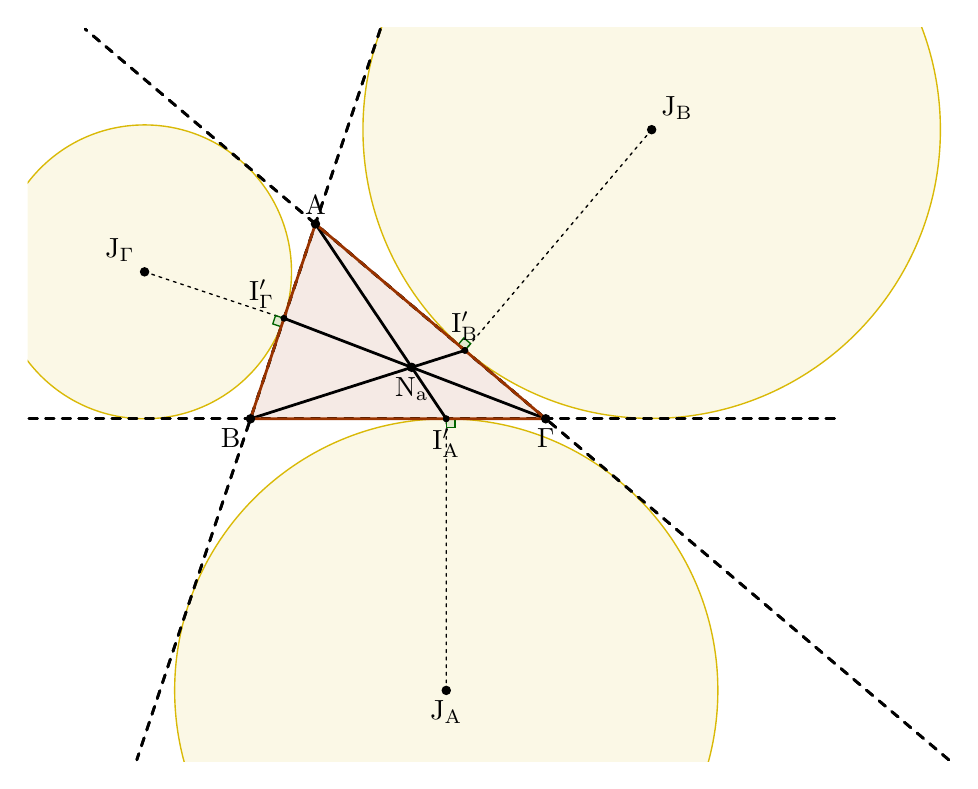
\begin{tikzpicture}[scale=.75]
\tkzSetUpLine[line width=1pt,color=black]
\tkzSetUpPoint[fill=black]

\tkzDefPoints{0/0/B,1.1/3.3/A,5/0/C}

\tkzDefSpcTriangle[ex](A,B,C){Ja,Jb,Jc}
\tkzDefSpcTriangle[extouch](A,B,C){Ta,Tb,Tc}
\tkzDefTriangleCenter[nagel](A,B,C)
\tkzGetPoint{Na}

\tkzFillPolygon[fill=ShapeClr,fill opacity=0.1](A,B,C)
\tkzDrawLines[add=0 and 0](A,Ta B,Tb C,Tc)
\tkzDrawPoints(Ja,Jb,Jc,Ta,Tb,Tc)
\tkzDrawLines[add=1 and 1.75,dashed](A,B)
\tkzDrawLines[add=0.75 and 1,dashed](B,C)
\tkzDrawLines[add=1.75 and 1,dashed](C,A)

\tkzClipBB
\tkzDrawCircles[line width=0.5pt,color=ParacircleClr,fill=ParacircleClr,fill opacity=0.1](Ja,Ta Jb,Tb Jc,Tc)

% Double draw these lines.
\tkzDrawLines[add=1 and 1.75,dashed](A,B)
\tkzDrawLines[add=0.75 and 1,dashed](B,C)
\tkzDrawLines[add=1.75 and 1,dashed](C,A)

\tkzDrawSegments[line width=0.5pt,color=black,dashed,dash pattern=on 1pt off 1.75pt](Ja,Ta Jb,Tb Jc,Tc)

\tkzMarkRightAngles[line width=0.5pt, size=.15,color=AngleClr,fill=AngleClr,fill opacity=0.1](Ja,Ta,C Jb,Tb,A Jc,Tc,B)

\tkzDrawPolygon[color=ShapeClr](A,B,C)

\tkzDrawPoints[size=3](Ja,Jb,Jc)
\tkzDrawPoints[size=2](Ta,Tb,Tc)
\tkzDrawPoints[size=3](B,C,A)
\tkzDrawPoints[size=3](Na)

\tkzLabelPoint[above](A){$\rm A$}
\tkzLabelPoint[below left](B){$\rm B$}
\tkzLabelPoint[below ](C){$\rm \Gamma$}
\tkzLabelPoint[below](Na){$\rm N_a$}

\tkzLabelPoint[below](Ta){$\rm I_A'$}
\tkzLabelPoint[above](Tb){$\rm I_B'$}
\tkzLabelPoint[above left](Tc){$\rm I_\Gamma'$}

\tkzLabelPoint[below](Ja){$\rm J_A$}
\tkzLabelPoint[above right](Jb){$\rm J_B$}
\tkzLabelPoint[above left](Jc){$\rm J_\Gamma$}


\end{tikzpicture}

\end{document}
